\begin{figure}[!htbp]
    \centering
    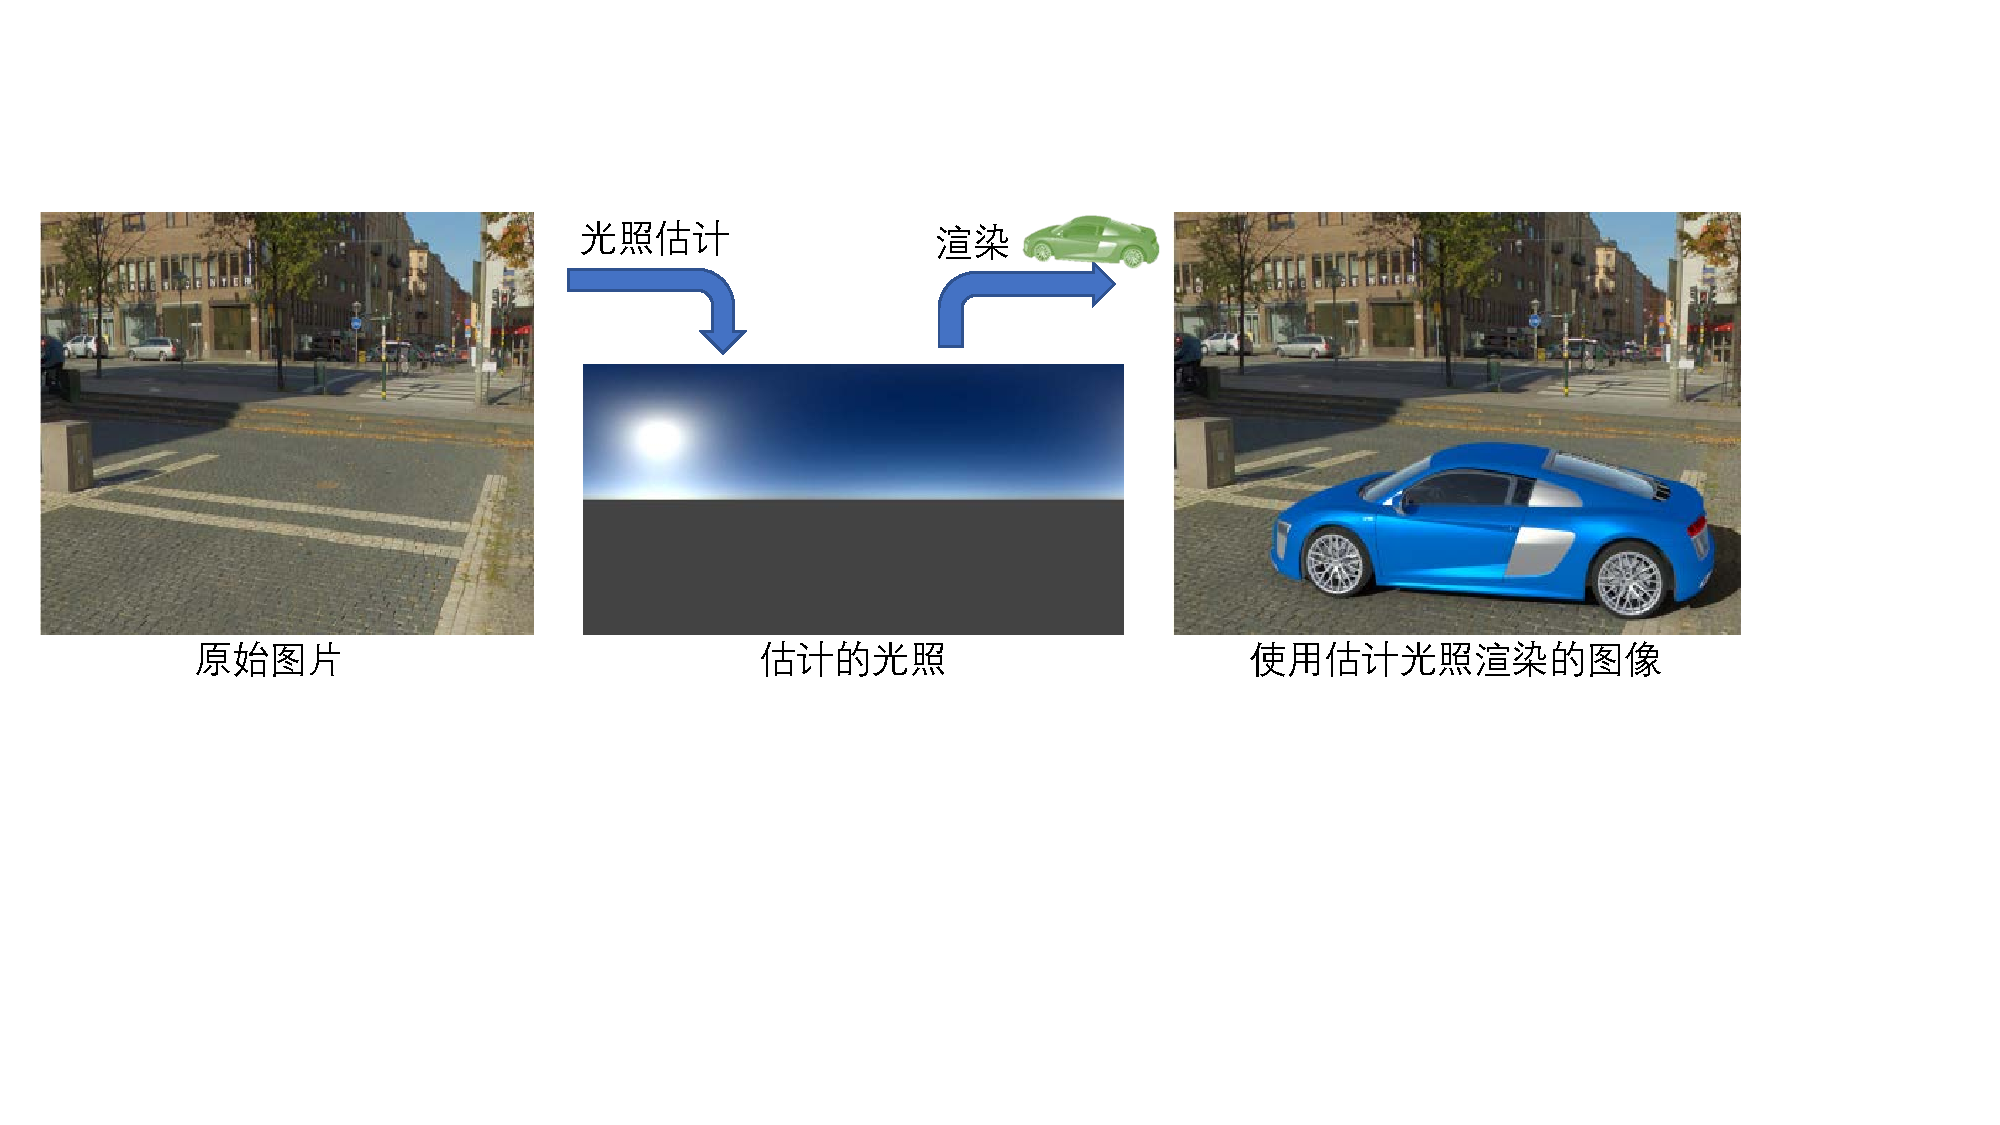
\includegraphics[width=1.0\textwidth]{Img/demo-problem-define.pdf}

    \caption[光照估计的应用]
    {光照估计的应用之一。使用单张图片估计场景的光照,并利用估计的光照渲染一个新的物体合成到图像中。
    可以看出使用估计光照渲染后的3D物体,与场景中的已有物体在视觉上较为一致。图片引自\cite{hold2017deep}。}
    % {3D rendering under the predicted illumination.
    % visual effect of the 3D rendering is in line with the original image.}
    
    \label{fig:demo-problem-define}
\end{figure}